%%%%%%%%%%%%%%%%%%%%%%%%%%%%%%%%%%%%%%%%%%%%%%%%%%%%%%%%%%%%%%%%%%%%%%%%%%%%%%%
% Chapter 3: Procedimiento experimental 
%%%%%%%%%%%%%%%%%%%%%%%%%%%%%%%%%%%%%%%%%%%%%%%%%%%%%%%%%%%%%%%%%%%%%%%%%%%%%%%



%++++++++++++++++++++++++++++++++++++++++++++++++++++++++++++++++++++++++++++++
\section{Descripci�n de los experimentos}
\label{3:sec:1}
Tras elaborar un programa en Python capaz de calcular la aproximaci�n de la funci�n ln(x) mediante la serie de Taylor y el tiempo que tarda la m�quina en realizar esa aproximaci�n,
hemos realizado varios experimentos fijando el punto,el centro o el grado. Adem�s,tambi�n elaboramos un programa que nos calcula el error de dicha aproximaci�n.
Los experimentos realizados son los siguientes: 
\begin{enumerate}
\item Fijamos el grado de la Serie de Taylor(n=10),el punto en el que deseamos que se aplique (x=4) y variamos el centro.
\item Fijamos el grado de la Serie de Taylor (n=8), el centro (c=6) y variamos el punto en el que deseamos que se aplique.
\item Fijamos el centro(c=1) , el punto en el que deseamos que se aplique la aproximaci�n (x=2) y variamos el grado.
\end{enumerate}
%++++++++++++++++++++++++++++++++++++++++++++++++++++++++++++++++++++++++++++++
\section{Descripci�n del material}
\label{3:sec:2}
Todos los experimentos realizados se han llevado a cabo en un ordenador con las siguientes caracter�sticas:
\begin{verbatim}
 - Sistema operativo : Linux, Ubuntu.
 - Procesador: Intel(R) Core(TM) i3 
 - CPU :  M 350  @ 2.27GHz 
\end{verbatim}
\clearpage
%++++++++++++++++++++++++++++++++++++++++++++++++++++++++++++++++++++++++++++++
\section{Resultados obtenidos}
\subsection{Funci�n real del Logartimo Neperiano}
\begin{figure}[!th]

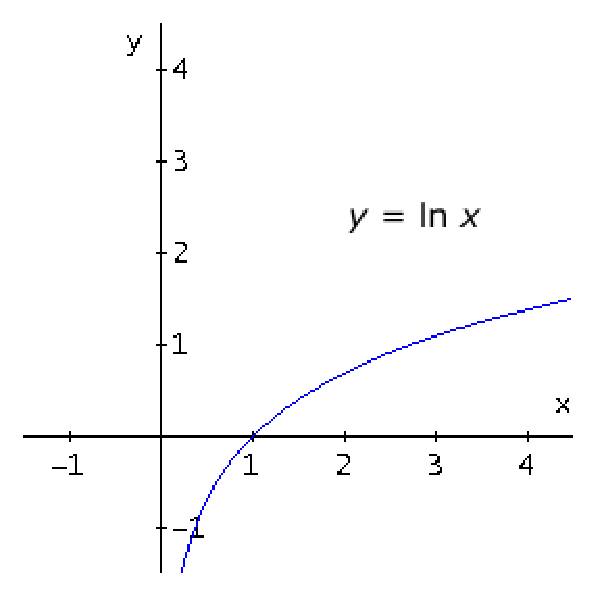
\includegraphics[width=0.30\textwidth]{images/fun053.eps}
\caption{Funci�n Logaritmo Neperiano}
\label{fig:1}

\end{figure}
\label{3:sec:3}

\subsection{Variaci�n del centro}
Fijando n=10 y x=4

\begin{tabular}{|l | r@{,}l |}
\hline
Si el valor de c= 2   & 1  & 33878210119487\\
\hline
Si el valor de c= 3   & 1  & 38629396788690\\
\hline 
Si el valor de c= 5   & 1  & 38629436340045\\
\hline
Si el valor de c= 30  & 1  & 48572417754861\\
\hline
Si el valor de c= 60  & 1  & 74292118557045\\
\hline
\end{tabular}


\subsection{Variaci�n del punto }
Fijando n=8 y c=6

\begin{tabular}{|l | r@{,}l |}
\hline
Si el valor de x= 8  &  2 & 07943719692636\\
\hline
Si el valor de x= 7  &  1 & 94591013946629\\
\hline
Si el valor de x= 6  &  1 & 79175946922805\\
\hline
Si el valor de x = 5 &  1 & 60943792540920\\
\hline
Si el valor de x= 4  & 1  & 38630243959407\\
\hline
\end{tabular}

\subsection{Variaci�n del grado }
Fijando x=2 y c=1

\begin{tabular}{|l | r@{,}l |}
\hline
Si el valor de n= 5     &  0 & 783333333333333\\
\hline
Si el valor de n= 15    &  0 & 725371850371850\\
\hline
Si el valor de n= 25    &  0 & 712747499542829\\
\hline
Si el valor de n= 200   &  0 & 690653430481824\\
\hline
Si el valor de n= 800   &  0 & 692522571184642\\
\hline
\end{tabular}
%------------------------------------------------------------------------------

%------------------------------------------------------------------------------

%++++++++++++++++++++++++++++++++++++++++++++++++++++++++++++++++++++++++++++++
\section{An�lisis de los resultados}
\label{3:sec:4}

\begin{itemize}
\item Variaci�n del centro: Variando el centro, fijando el grado (n=10) y el punto (x=4), podemos observar que cuanto m�s se aleja centro del punto menos acertado es el resultado.
\item Variaci�n del punto: Variando el punto, y fijando el centro (c=6) y el grado (n=8), observamos que si el punto es igual al centro el valor de la Serie de Taylor es  no conduce a ning�n error, ya que al ser iguales su diferencia es cero 
y nos da la imagen en ese punto o centro del logaritmo neperiano. Adem�s, vemos que si incrementamos la diferencia entre ambos puntos el resultado se aleja m�s del aut�ntico valor.
\item Variaci�n del grado: Al variar el grado y fijando el punto (x=2) y el centro (c=2), apreciamos que cuanto mayor es el grado m�s disminuye el error, por lo cual, si aunmentamos el valor del grado m�s precisos son los resultados. 
\end{itemize}
